%!TEX ROOT=ctutest.tex
\chapter{Úvod}
    
    Funkčnost a spolehlivost technických zařízení se výrazně podepisuje na provozních nákladech a bezpečnosti moderních systémů v průmyslu po celou dobu jejich fungování. 
    Za pomoci diagnostiky stavu zařízení a následné údržby je cílem každé firmy minimalizovat ztráty a rozsah škod způsobených jejich poruchami nebo úplným selháním. Tato diagnostika stavu a údržba zařízení je prováděna  všude kolem nás, ve všech technologických oblastech, od průmyslových zařízení, strojních a stavebních přístrojů, letecké techniky až po biotechnologická zařízení\ldots\\
    Na otázku, jak efektivně vyřešit poruchy nejrůznějších strojů, existuje jednoduchá odpověď – předejít jejím vznikům. Tato myšlenka nese filosofii konceptu údržby podle technického stavu (anglicky Condition Based Maintenance, dále jen jako CBM) a prediktivní údržby (Predictive Maintenence), které jsou jedním ze základních stavebních kamenů moderní diagnostiky zařízení v~průmyslu.
    
    Preventivní predeterminovaná údržba s pravidelnými kontrolami a diagnostikou stavu zařízení (anglicky Time Based Maintenance, dále jen TBM) byla po dlouhou dobu v minulosti nejspolehlivější metodou, jak předejít poruše stroje. V dnešní době, kdy je ale kladen důraz na maximální efektivitu, nese tento koncept údržby mnohá úskalí. Pravidelné kontroly zvyšují finanční náklady na provoz, mrhají jak lidskými tak materiálními zdroji, často musí kvůli nim být pozastavena výroba a navíc TBM zcela selhává při náhlých poruchách \cite{website:9}.
    
    Naproti tomu CBM díky mnoha moderním technologiím dnešní doby, které umožňují monitorovat a diagnostikovat stav zařízení v reálném čase, dokáže předvídat poruchu ještě před tím, než k ní dojde, a rozhoduje tak o provedení údržby v tu chvíli, kdy jí je opravdu třeba. Tento koncept je tedy proto v~mnoha aplikacích výhodnější, přináší časové, pracovní a materiálové úspory a je velice vhodný zejména pro zařízení, jejichž selhání má fatální následky \cite{website:9}.

\section{Diagnostika stavu rotačních zařízení}
    K selhání motorů může dojít mnoha způsoby. Fakta ale ukazují, že 40 až 90~\% poruch je zapříčiněno defektem ložisek \cite{book:1} a tyto poruchy navíc často způsobují selhání celého motoru.
    Monitorování jejich stavu se tedy stává důležitým úkolem a nejčastěji se k němu používá vibrační analýza a měření teploty. Tyto veličiny nejlépe reflektují stav ložisek – jejich mechanické namáhání, opotřebení materiálů či vznikající trhliny. Z vlastností vibračního signálu lze také identifikovat příznaky přicházejících poruch.\\
    Poruchami motorů a analýzou signálu se dále zabývá kapitola \ref{section:poruchy_mororu} a \ref{section:techniky}.
    
    \begin{figure} [!h]
        \centering
        \caption{Pracovník kontrolující stav motoru. Převzato z \cite{website:2}.}
            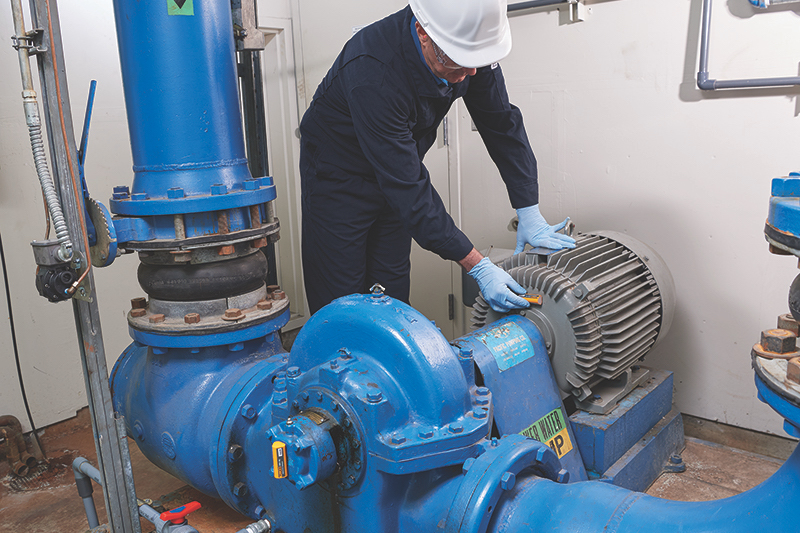
\includegraphics[width=0.8\textwidth]{INTRO/Figs/motor2.jpg}
    \end{figure} 
    
    

\section{Monitorování zařízení v rámci IIoT}
    Internet věcí (anglicky  Internet of Things, dále IoT) je jedním z fenoménů dnešního technologického světa. Pro mnohé se ale tento pojem stal symbolem své pouze jedné větve – spotřebitelského internetu věcí, který je z~popularizačního hlediska zajímavější, zaměřen na chytrá města a domácnosti.\\
    Stejný, ne-li vyšší význam, ale nese Průmyslový internet věcí (anglicky Industrial Internet of Things dále IIoT), často zaměňovaný s pojmem Průmysl 4.0. IIoT v~první řadě poskytuje lepší přehled o aktivitách v průmyslové výrobě a to prostřednictvím monitorujících senzorů, konektivity a cloud computingu.
     Díky zpětné vazbě získané z datové analýzy umožňuje transformovat a především optimalizovat výrobní operace, což zvyšuje zejména produktivitu, efektivitu a náklady \cite{article:1}.\\
     IIoT je tedy klíčovým faktorem umožňující realizovat moderní prediktivní údržbu a CBM.
    
    

\section{LPWAN a vibrační analýza}
    
    Bezdrátový IIoT představuje další větev Průmyslového Internetu věcí. Bezdrátové komunikační sítě se ale obzvláště v průmyslovém prostředí potýkají s řadu úskalí jako je například dovolená šířka pásma, EMC, spolehlivost komunikace a výdrž baterie. Většina dřívějších řídících a monitorovacích systémů ve výrobních halách využívala proto pro komunikaci již dobře dostupná rozhraní a protokoly jako průmyslový Ethernet, Fieldbus nebo HART (Highway Addressable Remote Transducer Protocol).\\
    V mnoha případech je ale použití drátových technologií příliš problematické. Konkrétně pro vibrační analýzu je třeba také uvažovat rotační zařízení pracující na obtížně dostupných místech, například v malých vodních elektrárnách, tunelech nebo na rozlehlých větrných elektrárnách. Funkčnost těchto zařízení ale bývá stěžejní, a proto je třeba je pravidelně monitorovat. Vytvoření drátové sítě by zde ovšem bylo velmi nákladné či úplně nemožné. V těchto případech je tedy nasnadě použít bezdrátové komunikační sítě LPWAN (Low Power Wide Area Network) jako například LoRa, SigFox či NB-IoT, jejichž dlouhý dosah, jednoduchá instalace a energetická nenáročnost představují hlavní argumenty jejich upřednostnění před ostatními komunikačními technologiemi.\\
    Postavením LPWAN sítí v rámci IIoT se dále zabývá kapitola \ref{section:lpwan}.
    
%CHECK ~
%CHECK red
%CHECK ...